\chapter{Proyecto de Ruby on Rails}

\section{Fase de análisis}

\subsection{Requisitos funcionales}

\begin{itemize}
	\item
		Se debe poder registrar un usuario.
		\begin{itemize}
			\item
				Un usuario registrado debe poder iniciar sesión.
			\item
				Un usuario con sesión iniciada debe poder terminarla.
			\item
				Los usuarios deben estar registrados para interactuar con el sistema.
		\end{itemize}
	\item
		El servidor almacena el estado del juego de los usuarios.
	\item
		Los jugadores desbloquean logros con sus acciones.
		\begin{itemize}
			\item
				Los logros aportan experiencia al jugador.
			\item
				El jugador tiene un nivel calculado por su experiencia.
		\end{itemize}
	\item
		Existe una \textit{wiki} en la que consultar el manual de usuario del juego.
		\begin{itemize}
			\item
				La \textit{wiki} es accesible desde la página web.
			\item
				Los logros están documentados en la \textit{wiki}.
			\item
				La \textit{wiki} implementa un motor de búsqueda.
		\end{itemize}
	\item
		Se puede el perfil de los diferentes usuarios
		\begin{itemize}
			\item
				El perfil del propio usuario ofrece herramientas de edición de la cuenta.
		\end{itemize}
	\item
		Se puede consultar un \textit{ranking} de los jugadores con más experiencia.
\end{itemize}

\subsection{Requisitos no funcionales}

\begin{itemize}
	\item
		Licencia GPL-3.0
	\item
		El acceso a la base de datos debe ser eficiente.
	\item
		El acceso a la base de datos debe ser seguro.
	\item
		Las fuentes utilizadas en la web deben ser fácilmente legibles.
	\item
		La página web debe ser ligera para todos los dispositivos.
\end{itemize}

\subsection{Partes interesadas y preocupaciones}

\begin{itemize}
	\item
		\textbf{Usuarios del juego:}
		Quieren disfrutar de la experiencia que ofrecemos.
	\item
		\textbf{Desarrolladores:}
		Quieren aprobar la asignatura.
	\item
		\textbf{Comunidad \textit{open source}:}
		Quieren aprender sobre cómo hemos trabajado y expandir las funcionalidades del sistema.
	\item
		\textbf{Inversores:}
		Ven una posibilidad de introducir elementos en el juego que les genere beneficio.
\end{itemize}

\subsection{Diagrama arquitectónico}

\begin{figure}[!ht]
\begin{center}
	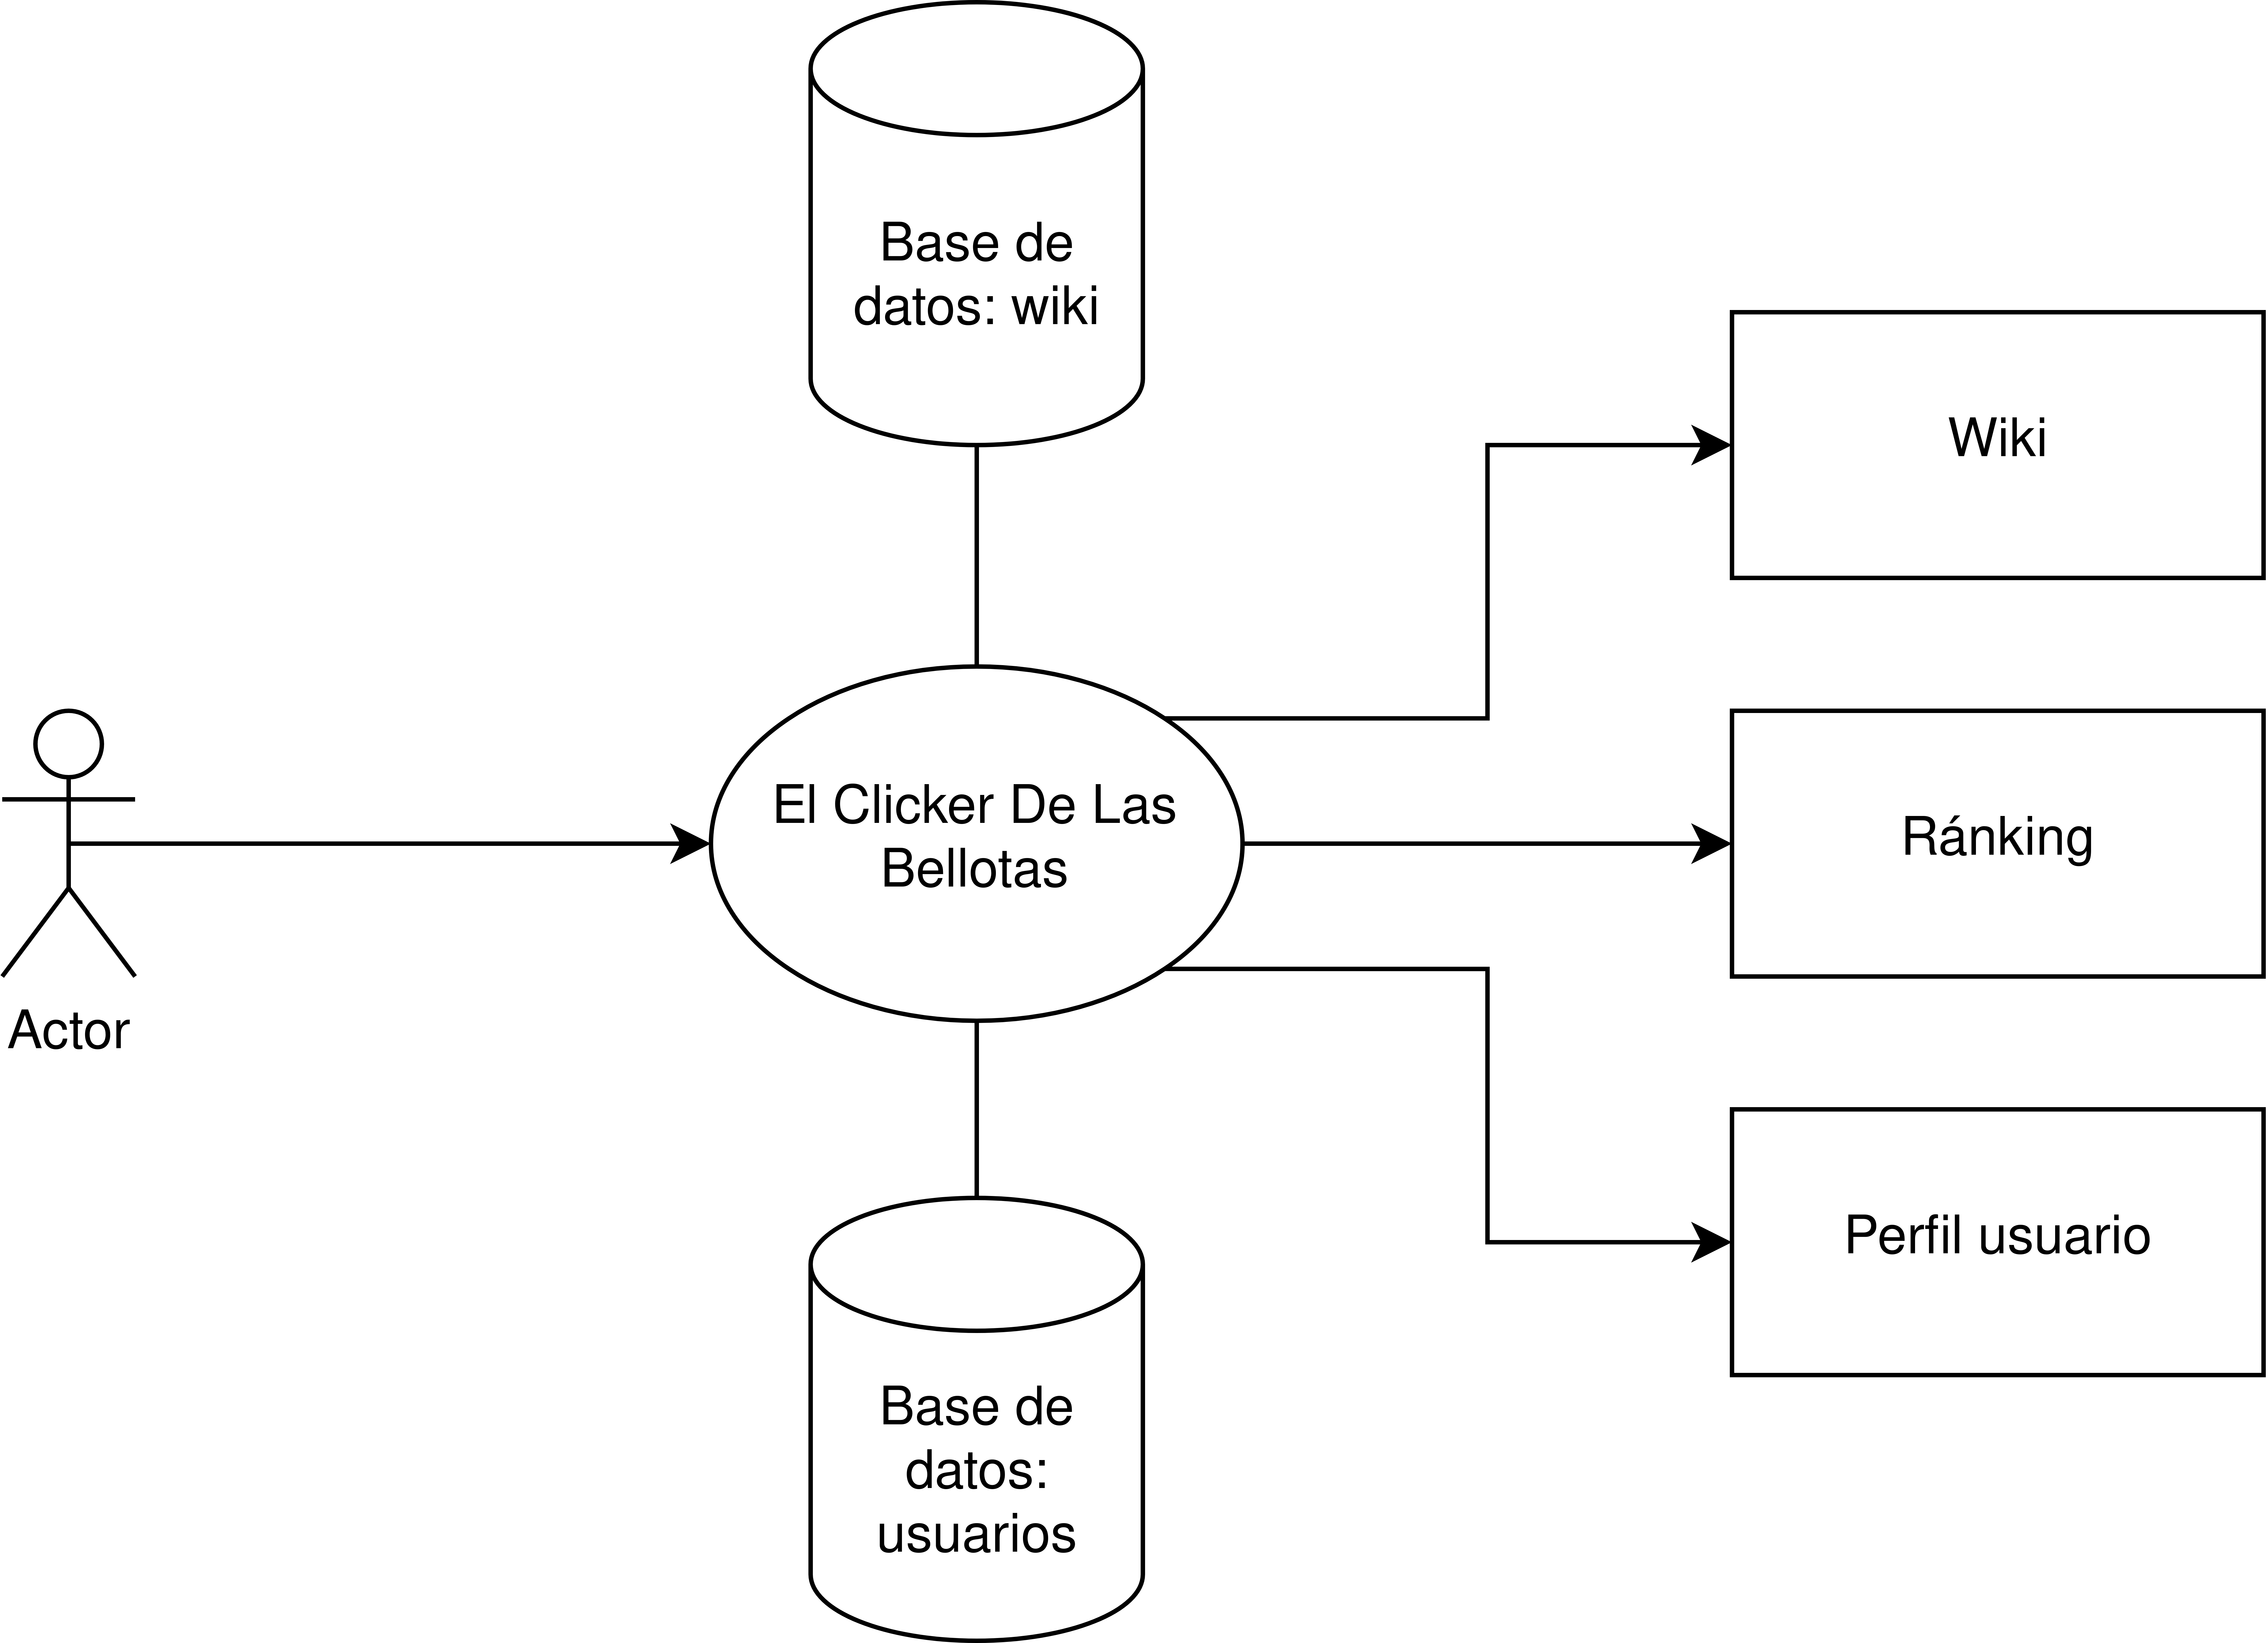
\includegraphics[scale=0.75]{Diagrama de contexto}
\end{center}
\caption{Diagrama de contexto de nuestra aplicación}
\end{figure}

\subsection{Criterios de calidad}

\begin{itemize}
	\item
		Los datos de los usuarios deben estar protegidos contra ataques que violen su privacidad.
	\item
		El sistema debe cumplir en todo momento con las indiciaciones de las ESRB y PEGI\@.
	\item
		Los accesos a la base de datos deben ser fiables.
	\item
		Todo el código y el acceso al sistema debe ser libre.
\end{itemize}

\section{Fase de diseño}

\subsection{Diagrama de clases}
